
\let\negmedspace\undefined
\let\negthickspace\undefined
\documentclass[journal,12pt,onecolumn]{IEEEtran}
\usepackage{cite}
\usepackage{amsmath,amssymb,amsfonts,amsthm}
\usepackage{algorithmic}
\usepackage{graphicx}
\graphicspath{{./figs/}}
\usepackage{textcomp}
\usepackage{xcolor}
\usepackage{txfonts}
\usepackage{listings}
\usepackage{enumitem}
\usepackage{mathtools}
\usepackage{gensymb}
\usepackage{comment}
\usepackage{caption}
\usepackage[breaklinks=true]{hyperref}
\usepackage{tkz-euclide} 
\usepackage{listings}
\usepackage{gvv}                                        
%\def\inputGnumericTable{}                                 
\usepackage[latin1]{inputenc}     
\usepackage{xparse}
\usepackage{color}                                            
\usepackage{array}                                            
\usepackage{longtable}                                       
\usepackage{calc}                                             
\usepackage{multirow}
\usepackage{multicol}
\usepackage{hhline}                                           
\usepackage{ifthen}                                           
\usepackage{lscape}
\usepackage{tabularx}
\usepackage{array}
\usepackage{float}
%\newtheorem{theorem}{Theorem}[section]
%\newtheorem{theorem}{Theorem}[section]
%\newtheorem{problem}{Problem}
%\newtheorem{proposition}{Proposition}[section]
%\newtheorem{lemma}{Lemma}[section]
%\newtheorem{corollary}[theorem]{Corollary}
%\newtheorem{example}{Example}[section]
%\newtheorem{definition}[problem]{Definition}

\begin{document}

%\textbf{\Large 2.6.38} \\
%\textbf{\large AI25BTECH11027 - NAGA BHUVANA} \\
\title{4.4.23}
\author{AI25BTECH11027 - NAGA BHUVANA}
% \maketitle
% \newpage
% \bigskip
%\begin{document}
{\let\newpage\relax\maketitle}
%\renewcommand{\thefigure}{\theenumi}
%\renewcommand{\thetable}{\theenumi}
\noindent
		\textbf{Question:}\\
If the graph of a pair of lines $x-2y+3=0$ and $2x-4y=5$ be drawn,that what type of lines are drawn?\\
\textbf{Solution:}\\
\begin{align}
    \vec{A}=\myvec{1&-2\\2&-4} , \vec{b}=\myvec{-3\\5}
\end{align}
Consider the augmented matrix $\vec{M}=\myvec{\vec{A} & \vec{b}}$
        \begin{align}
            \vec{M}=\myvec{1&-2 & -3\\2 &-4 & 5}
        \end{align}
        By doing Row operation $R_2 \longleftarrow R_2-2R_1$
        \begin{align}
            \vec{M}=\myvec{1&-2&-3\\0&0&11}
        \end{align}
        \begin{align}
            0x+0y=11
        \end{align}
        The above equations have no solution and the lines are \textbf{Parallel}\\
	\begin{figure}[H]
	\centering
	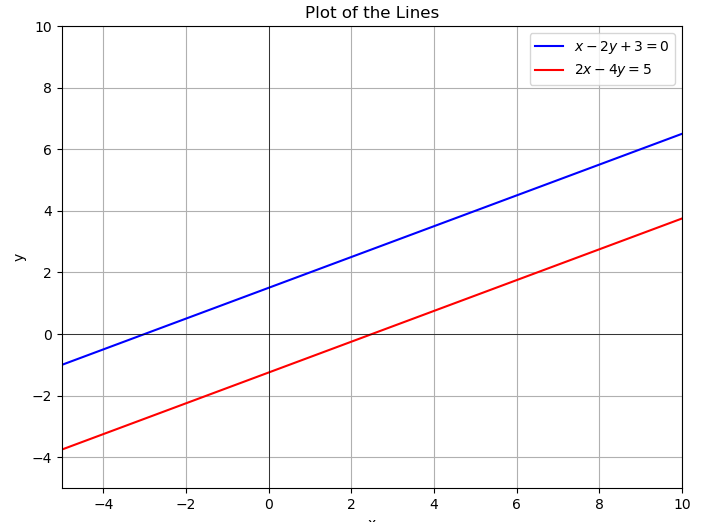
\includegraphics[width=0.7\linewidth]{figs/fig1.png}
	\caption{}
	\label{fig}
	\end{figure}
\end{document}
